\documentclass[tikz,border=5pt]{standalone}
\usepackage[utf8]{inputenc}
\usepackage[T1]{fontenc}
\usepackage{lmodern,amsmath,amssymb}
\usepackage[american]{circuitikz}
\usepackage{pgfplots}
\pgfplotsset{compat=1.18}
\usetikzlibrary{circuits.logic.US,positioning,calc,arrows.meta,patterns,shapes.geometric}
\definecolor{Primary}{HTML}{1F77B4}
\begin{document}
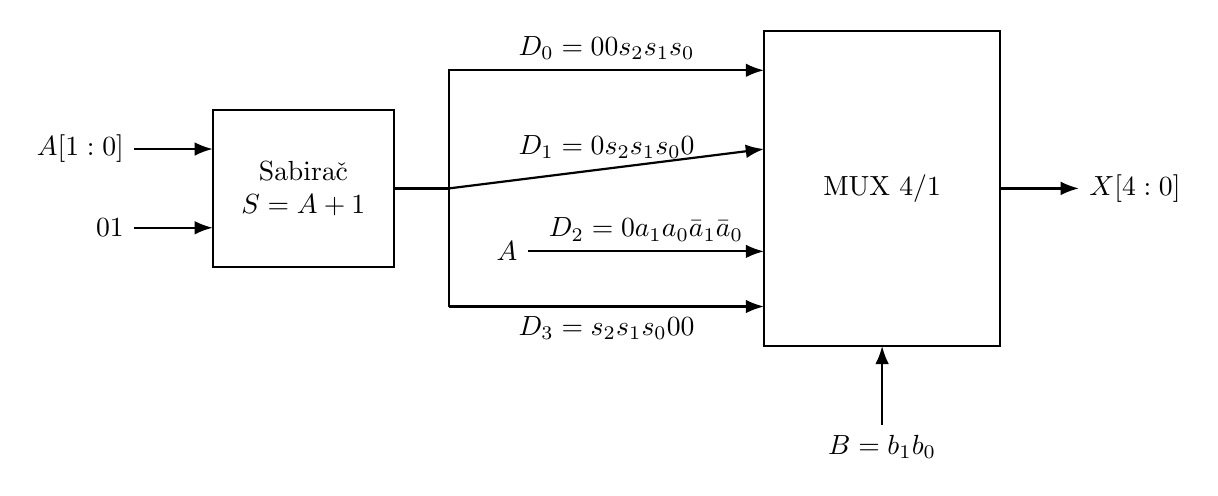
\begin{tikzpicture}[thick,>=Latex]
\draw(0,0)rectangle(2.3,2);\node[align=center]at(1.15,1){Sabirač\\$S=A+1$};\draw[->](-1,1.5)node[left]{$A[1:0]$}--(0,1.5);\draw[->](-1,.5)node[left]{$01$}--(0,.5);
\draw(7,-1)rectangle(10,3);\node at(8.5,1){MUX 4/1};
\draw[->](2.3,1)--(3,1)--(3,2.5)--(7,2.5)node[midway,above]{$D_0=00s_2s_1s_0$};
\draw[->](3,1)--(7,1.5)node[midway,above]{$D_1=0s_2s_1s_00$};
\draw[->](3,-.5)--(7,-.5)node[midway,below]{$D_3=s_2s_1s_000$};\draw(3,1)--(3,-.5);
\draw[->](4,.2)node[left]{$A$}--(7,.2)node[midway,above]{$D_2=0a_1a_0\bar a_1\bar a_0$};
\draw[->](8.5,-2)node[below]{$B=b_1b_0$}--(8.5,-1);\draw[->](10,1)--(11,1)node[right]{$X[4:0]$};
\end{tikzpicture}
\end{document}
